\newpage
\section{Configuración  de TeXstudio}

Para poder procesar correctamente la bilbiografía en \LaTeX\ hay que ajustar el orden de compilación por defecto que viene en cualquier programa que trabaje con archivos \verb|.tex|. En este caso, se muestra el ejemplo con TeXstudio.

Lo que hay que hacer es ir a \verb|Opciones > Configurar TeXstudio| y dentro de la pestaña \verb|Compilar| se debe ajustar los comandos de \verb|Compilador por defecto| y \verb|Herramienta|  \verb|bibliográfica por defecto|. Para el primer caso, se hace clic en el botón \verb|Configurar| y se debe dejar la siguiente secuencia de órdenes: 
\begin{center}
	\verb|PdfLaTeX > Biber > PdfLaTeX > PdfLaTeX|.
\end{center}
Para el caso de bibliografía solo debe tener la órden de \verb|Biber|. En las siguientes figuras se indica como debería quedar configurado.
\begin{figure}[h]
	\centering
	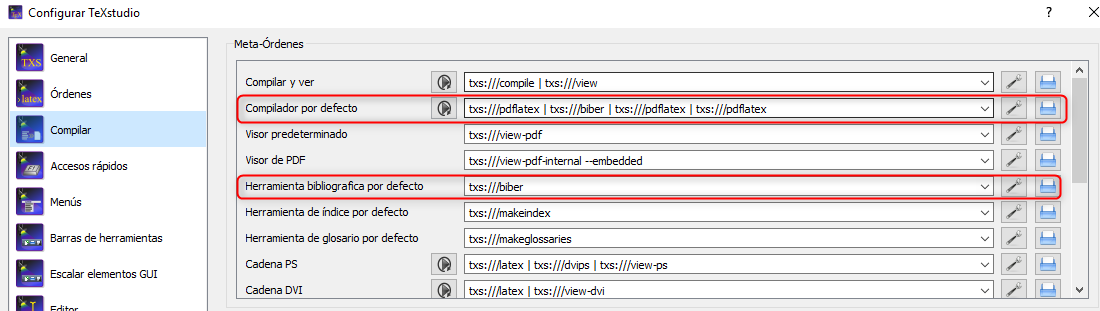
\includegraphics[width=1\linewidth]{compilar_1}
	\caption{Configuración de compilación en TeXstudio.}
	\label{fig:compilar1}
\end{figure}

\begin{figure}[h]
	\centering
	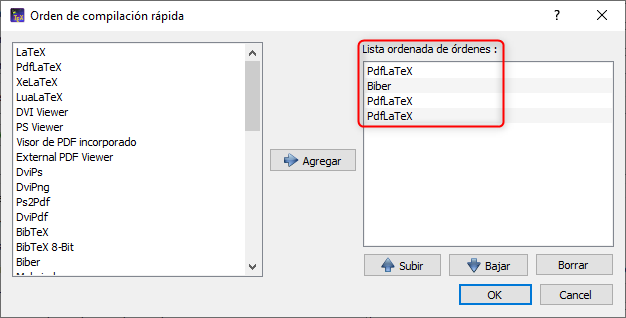
\includegraphics[width=0.7\linewidth]{compilar_2}
	\caption{Secuencia de órdenes de compilación.}
	\label{fig:compilar2}
\end{figure}

\newpage




